\subsection{Durchführung}

Im ersten Versuchsteil wird die Winkelverteilung der Höhenstrahlung gemessen. Dazu werden 24 Detektoren (Z1-Z24) kreisförmig angeordnet und ein zusätzlicher Detektor (Z25) in die Mitte des Kreises gestellt (siehe Abb. \ref{fig:winkel_skizze}). Jeder Detektor ist mit einem Diskriminator verbunden, der ab einer bestimmten Schwelle einen Puls abgibt (Längen der Pulse: Oben: \SI{30}{\nano\second}, Unten: \SI{50}{\nano\second}, Z25: \SI{100}{\nano\second}).
Geben gleichzeitig drei Detektoren, die auf einer Linie liegen ein Signal, so wird diese Koinzidenz als Teilchendurchgang identifiziert. Man zählt nun über einen bestimmten Zeitraum die Anzahl der Koinzidenzen aus allen Richtungen und erhält somit die Verteilung der Höhenstrahlung.

\begin{figure}[h]
\centering
\includegraphics[scale=0.9]{img/winkel_skizze.png}
\caption{Anordnung der Detektoren\cite{praktikumsheft}}
\label{fig:winkel_skizze}
\end{figure}

\subsubsection{Schwellenkurve}
Bevor man die Winkelverteilung messen kann, muss zuerst die optimale Schwelle für den Diskriminator D12 bestimmt werden. Die Schwellen der anderen Diskrimatoren sind schon eingestellt. Dazu wird die Schwelle des Diskrimators von -50 bis  \SI{-250}{\milli\volt} in \SI{10}{\milli\volt} Schritten verändert und jeweils für \SI{2520}{\second} die Anzahl der Koinzidenzen von D12 mit D23, D24, D1 oder D2 gemessen. Dies wird über ein LabVIEW-Programm automatisiert (siehe Abb. \ref{fig:prog_all}).\\

Im ersten Teil des Programms wird die Hardware initialisiert (siehe Abb. \ref{fig:prog_init}). Im Wesentlichen werden die Diskrimatoren D12 (Id 3), D23, D24, D1, D2 (Ids 1, 4, 5, 7) und D25 (Id 7) mit einer LED verbunden. Danach wird das ODER-Signal aus den Signalen D23, D24, D1 und D2 ermittelt, indem man sie über Oder-Blöcke verknüpft. Das Ausgangssignal wird wieder auf eine LED gegeben. Um Signale zu zählen werden Koinzidenzzähler verwendet. Zähler 1 zählt Koinzidenzen aus D12 und dem ODER-Signal, Zähler 2 die Anzahl der Signale in D12, Zähler 3 die ODER-Signale und Zähler 4 die Signale aus D25. \\

Der zweite Teil besteht aus zwei verschachtelten Schleifen (siehe Abb. \ref{fig:prog_prog}). Vor der äußeren Schleife wird die Schwelle auf einen Startwert gesetzt (\SI{-50}{\milli\volt}) und fünf Arrays initialisiert (eines, um die Schwellenwerte zu speichern und die anderen vier für die Anzahl der Ereignisse in den Koinzidenzzählern). Die äußere Schleife setzt den Schwellenwert des Diskriminators und speichert ihn im Array, wartet dann \SI{2520}{\second} und fügt dann die gemessenen Koinzidenzen der einzelnen Koinzidenzzähler an die jeweiligen Arrays ein. Danach werden die Zähler zurückgesetzt und die Schwelle um \SI{10}{\milli\volt} verringert, bis \SI{-250}{\milli\volt} erreicht wurden.\\
Die innere Schleife ist im wesentlichen dazu da, um die \SI{2520}{\second} zu warten. Parallel dazu werden die jeweiligen Zählraten im Interaktionsfenster von LabVIEW angezeigt.\\
Zum Schluss des Programms werden alle Arrays zusammengefasst und in eine Datei geschrieben.

\begin{figure}[h]
\centering
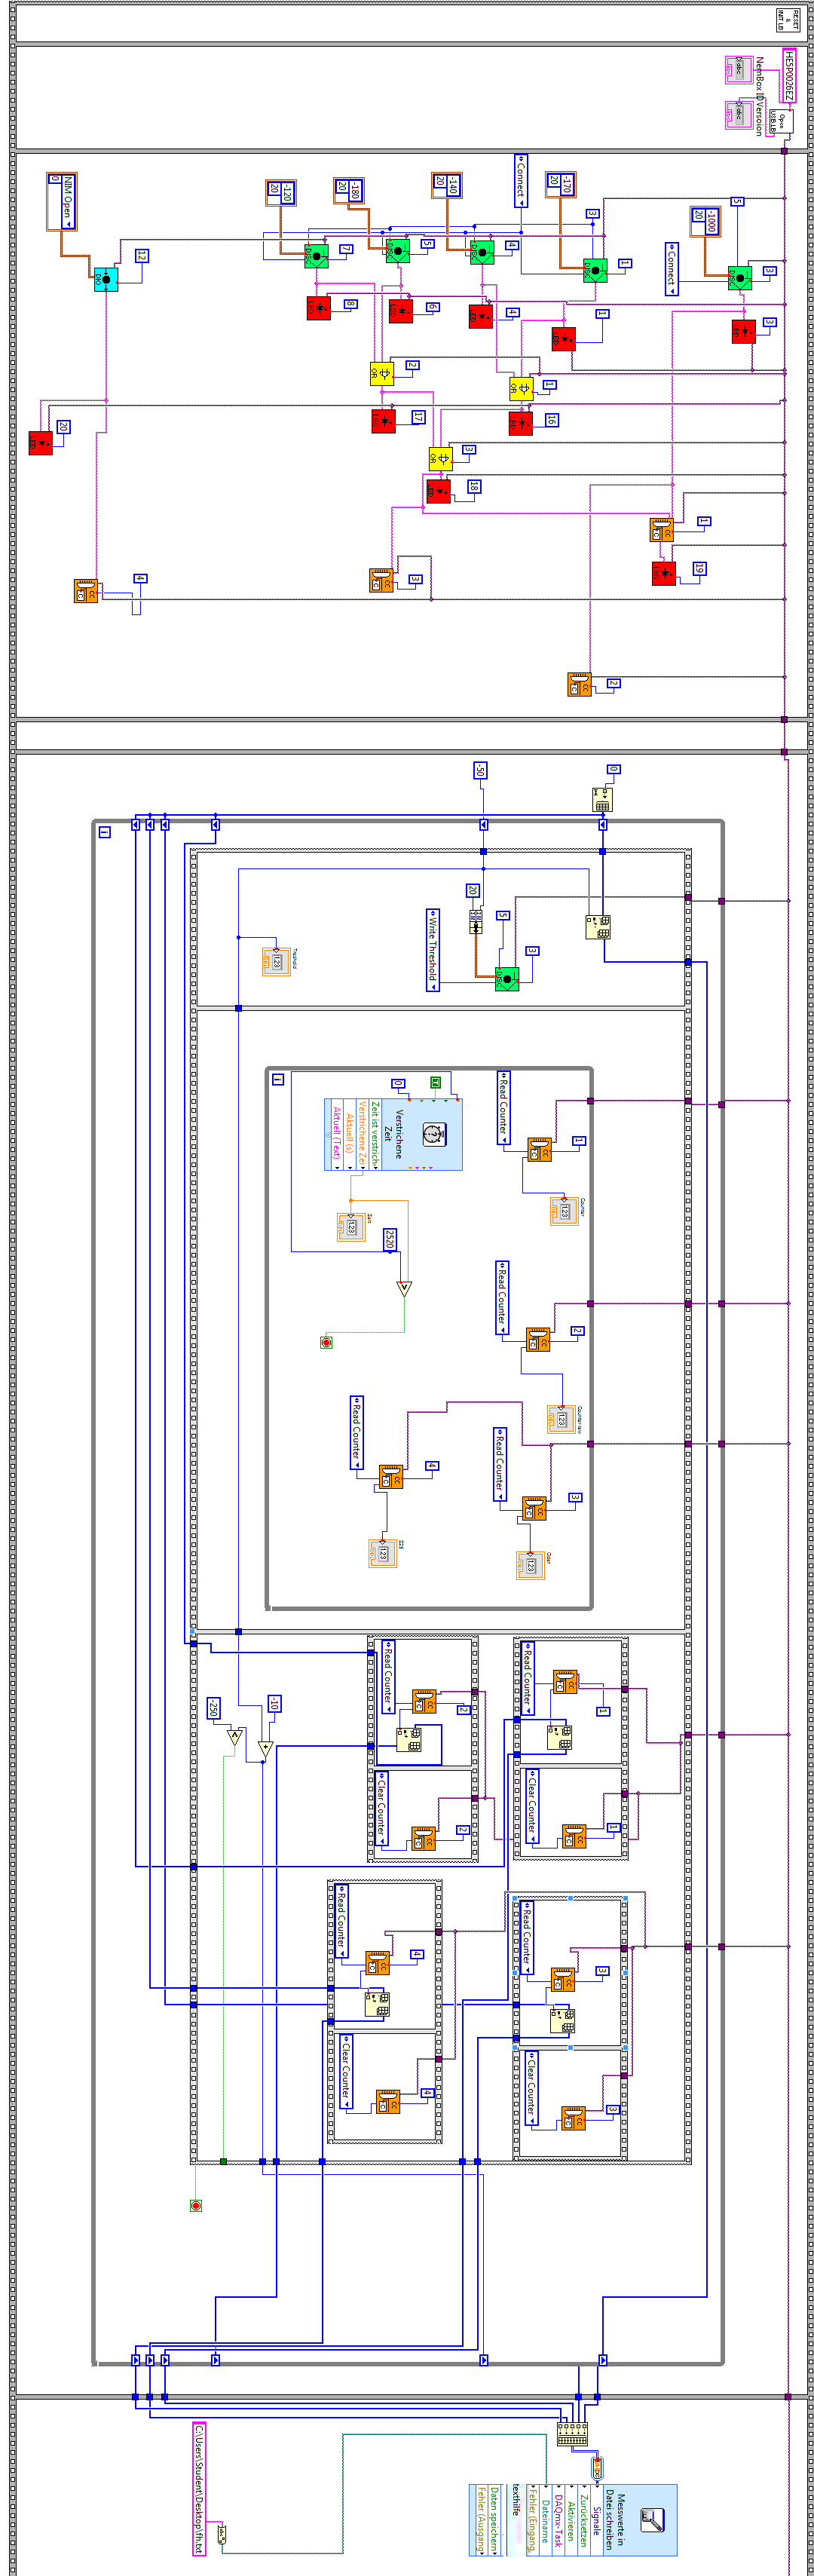
\includegraphics[height=20cm]{data/friedrich/prog_ges_rot.png}
\caption{Gesamtes Programm}
\label{fig:prog_all}
\end{figure}

\begin{figure}[h]
\centering
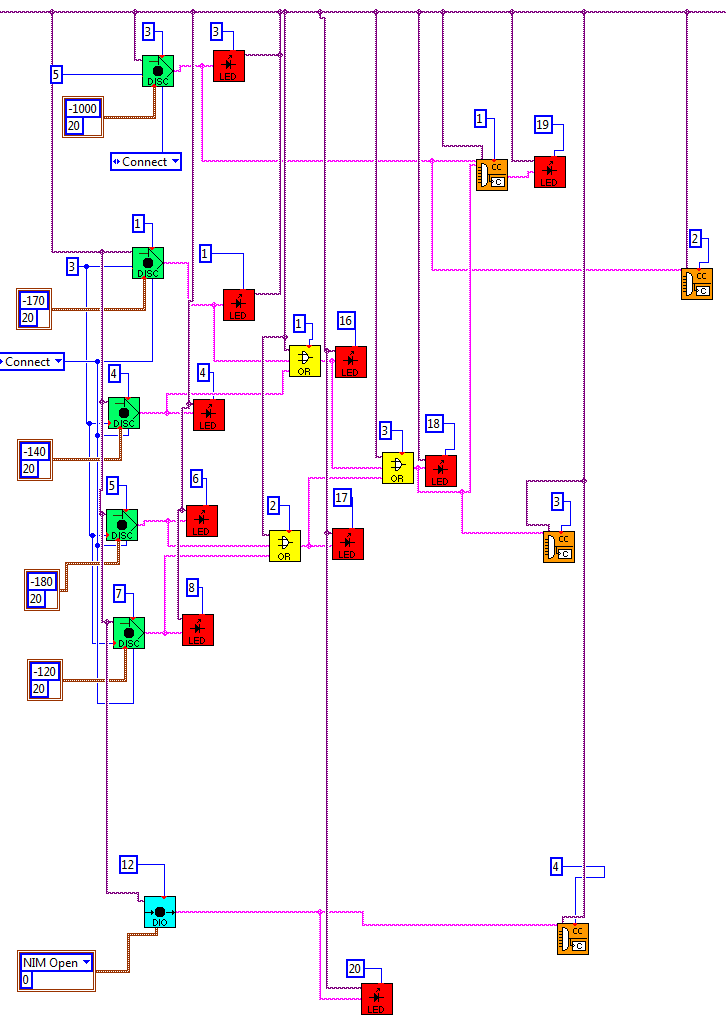
\includegraphics[height=20cm]{data/friedrich/prog_init.png}
\caption{Hardwareinitialisierung}
\label{fig:prog_init}
\end{figure}

\begin{figure}
\centering
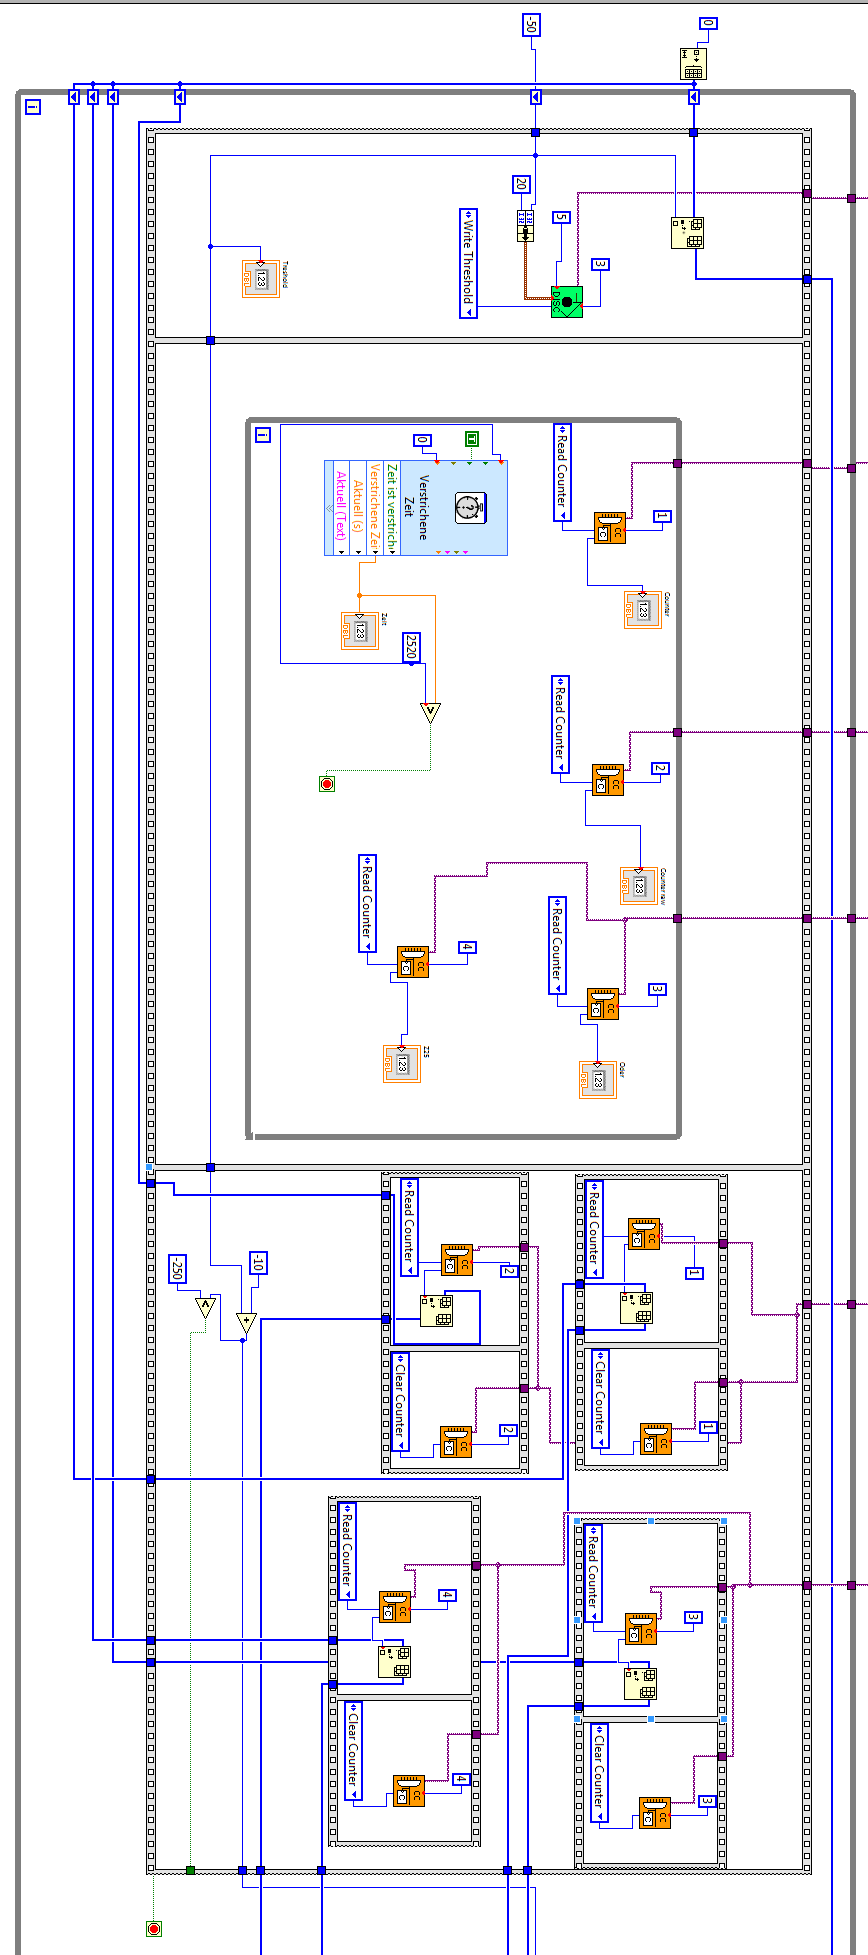
\includegraphics[height=20cm]{data/friedrich/prog_prog_rot.png}
\caption{Hauptprogramm}
\label{fig:prog_prog}
\end{figure}

\FloatBarrier

\subsubsection{Zufallskoinzidenzen}
Zusätzlich zur eigentlichen Messung wird versucht die Häufigkeit von Zufallskoinzidenzen zu messen. Dies geschieht auf 2 Arten.
\begin{itemize}
	\item Räumliche Zufallskoinzidenzen: Die Koinzidenzen von Detektor Z11, Z14 und Z25 werden gezählt. Solche Koinzidenzen werden z.B. verursacht von Teilchen, die nur in 2 Detektoren ein Signal auslösen, aber zufällig ein weiteres Signal in dem letzten Detektor erzeugt wird. Geht man von einem Teilchen aus, dass z.B. durch Z11 und Z25 geflogen ist, dann wird eine zufällige Koinzidenz erkannt, wenn 50ns davor oder danach ein Signal aus Z14 kommt. Die erwartete Anzahl beträgt also bei insgesamt N Ereignisse und einer Messdauer $t$ etwa: 
\begin{align}
N_{\text{raum}} = N \cdot \frac{\SI{100}{\nano\second}}{t} \cdot N = \frac{\SI{100}{\nano\second}}{t} \cdot N^2 
\label{equ:random_space}
\end{align}

	\item Zeitliche Zufallskoinzidenzen: Die Signale von Z2, Z14 und Z25 werden so verzögert, dass ein Teilchen keine Koinzidenz mehr erzeugen kann. Die Koinzidenzen, die dann gemessen werden, entsprechen 3 zufälligen Signalen in den Detektoren. Für eine Koinzidenz muss nun nicht nur ein Ereignis zufällig $\SI{50}{\nano \second}$ vor oder $\SI{100}{\nano \second}$ nach dem Z25 Signal passiert sein, sondern auch noch ein weiteres Signal $\SI{30}{\nano \second}$ vorher oder $\SI{50}{\nano \second}$ danach. Die Rate beträgt also etwa:
	\begin{align}
N_{\text{zeit}} = N \cdot \frac{\SI{150}{\nano\second}}{t} \cdot N \cdot \frac{\SI{80}{\nano\second}}{t} \cdot N = \frac{\SI{12000}{\nano\second}^2}{t^2}N^3
\label{equ:random_time}
\end{align}

\end{itemize}

\subsubsection{Pulshöhenspektrum}
Weiterhin wird auch noch die Energieverteilung der Teilchen in Z12 gemessen. Der Aufbau ist dabei so ähnlich wie bei der Messung der Schwellenkurve. Wieder zählen nur Ereignisse, die eine Koinzidenz aus D12 und D23, D24, D1 oder D2 darstellen. Kommt es zu einer solchen Koinzidenz wird das Signal in Z12 an einen MCA weitergeleitet, der die Ereignisse nach der Energie sortiert.
